We call {\em focus-inversive} (or simply {\em inversive}) the family of triangles which are the inversive image of billiard N-periodics with respect to a circle centered on a focus. The $N=3$ case is shown in \cref{fig:08-n3-finv}.

Note that since the inversive image of an ellipse with respect to a focus is a loopless Pascal's Limaçon, see \cite{mw}, the focus-inversive is inscribed in such a curve ans is therefore not Ponceletian. Indeed, the caustic is also non-elliptic. As shown in \cref{fig:08-n3-caustics}, a continuously increasing billiard aspect ratio will transition the caustic from (i) a regular curve, to (ii) one with a self-intersection and two cusps, to (iii) a non-compact curve with two infinite branches.

\begin{figure}
    \centering
    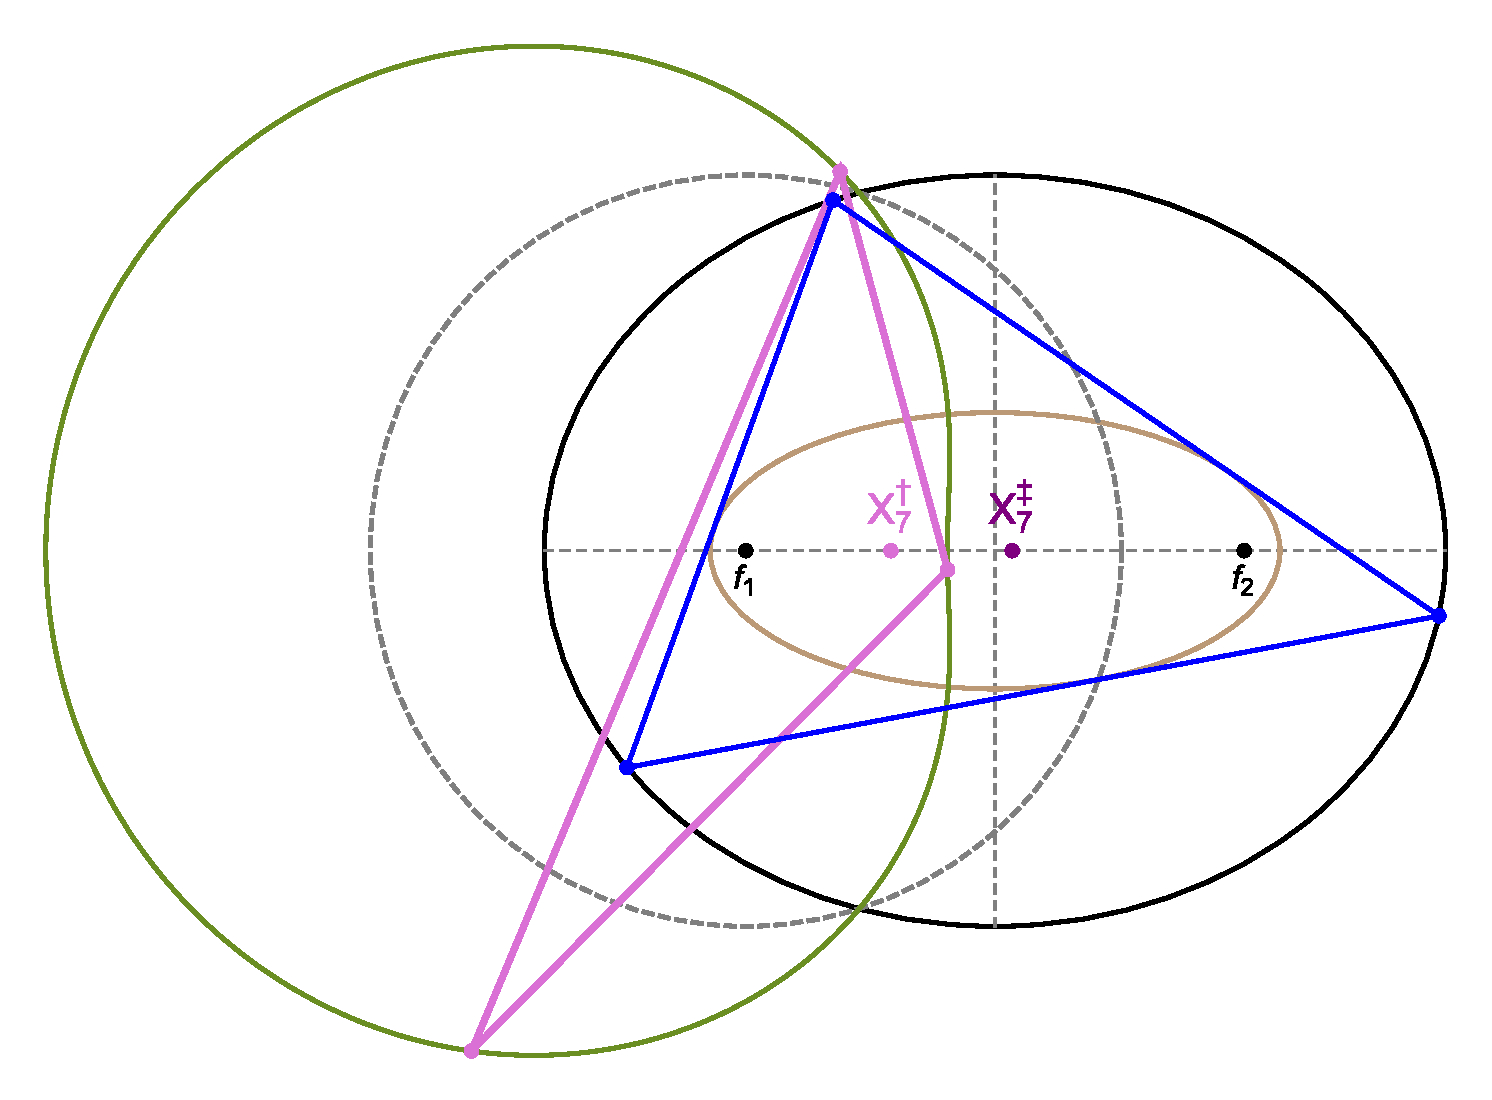
\includegraphics[width=.8\textwidth]{pics_08_010_n3_finv.eps}
    \caption{The $N=3$ focus-inversive family (pink), i.e., the inversive image of billiard 3-periodics (blue) with respect to a focused-centered circle $\Cm$ (dashed gray). Focus-inversives are inscribed in a loopless Pascal's Limaçon (olive green). Both perimeter and sum of cosines are invariant. The Gergonne point $X_7^\dagger$ is stationary. Also shown is $X_7^\ddagger$, the inversive image of $X_7^\dagger$ with respect to $\Cm$, inquired about in \cref{exe:08-x7-ddagger}. \href{https://bit.ly/3i19g6Q}{Live}}
    \label{fig:08-n3-finv}
\end{figure}

\begin{figure}
    \centering
    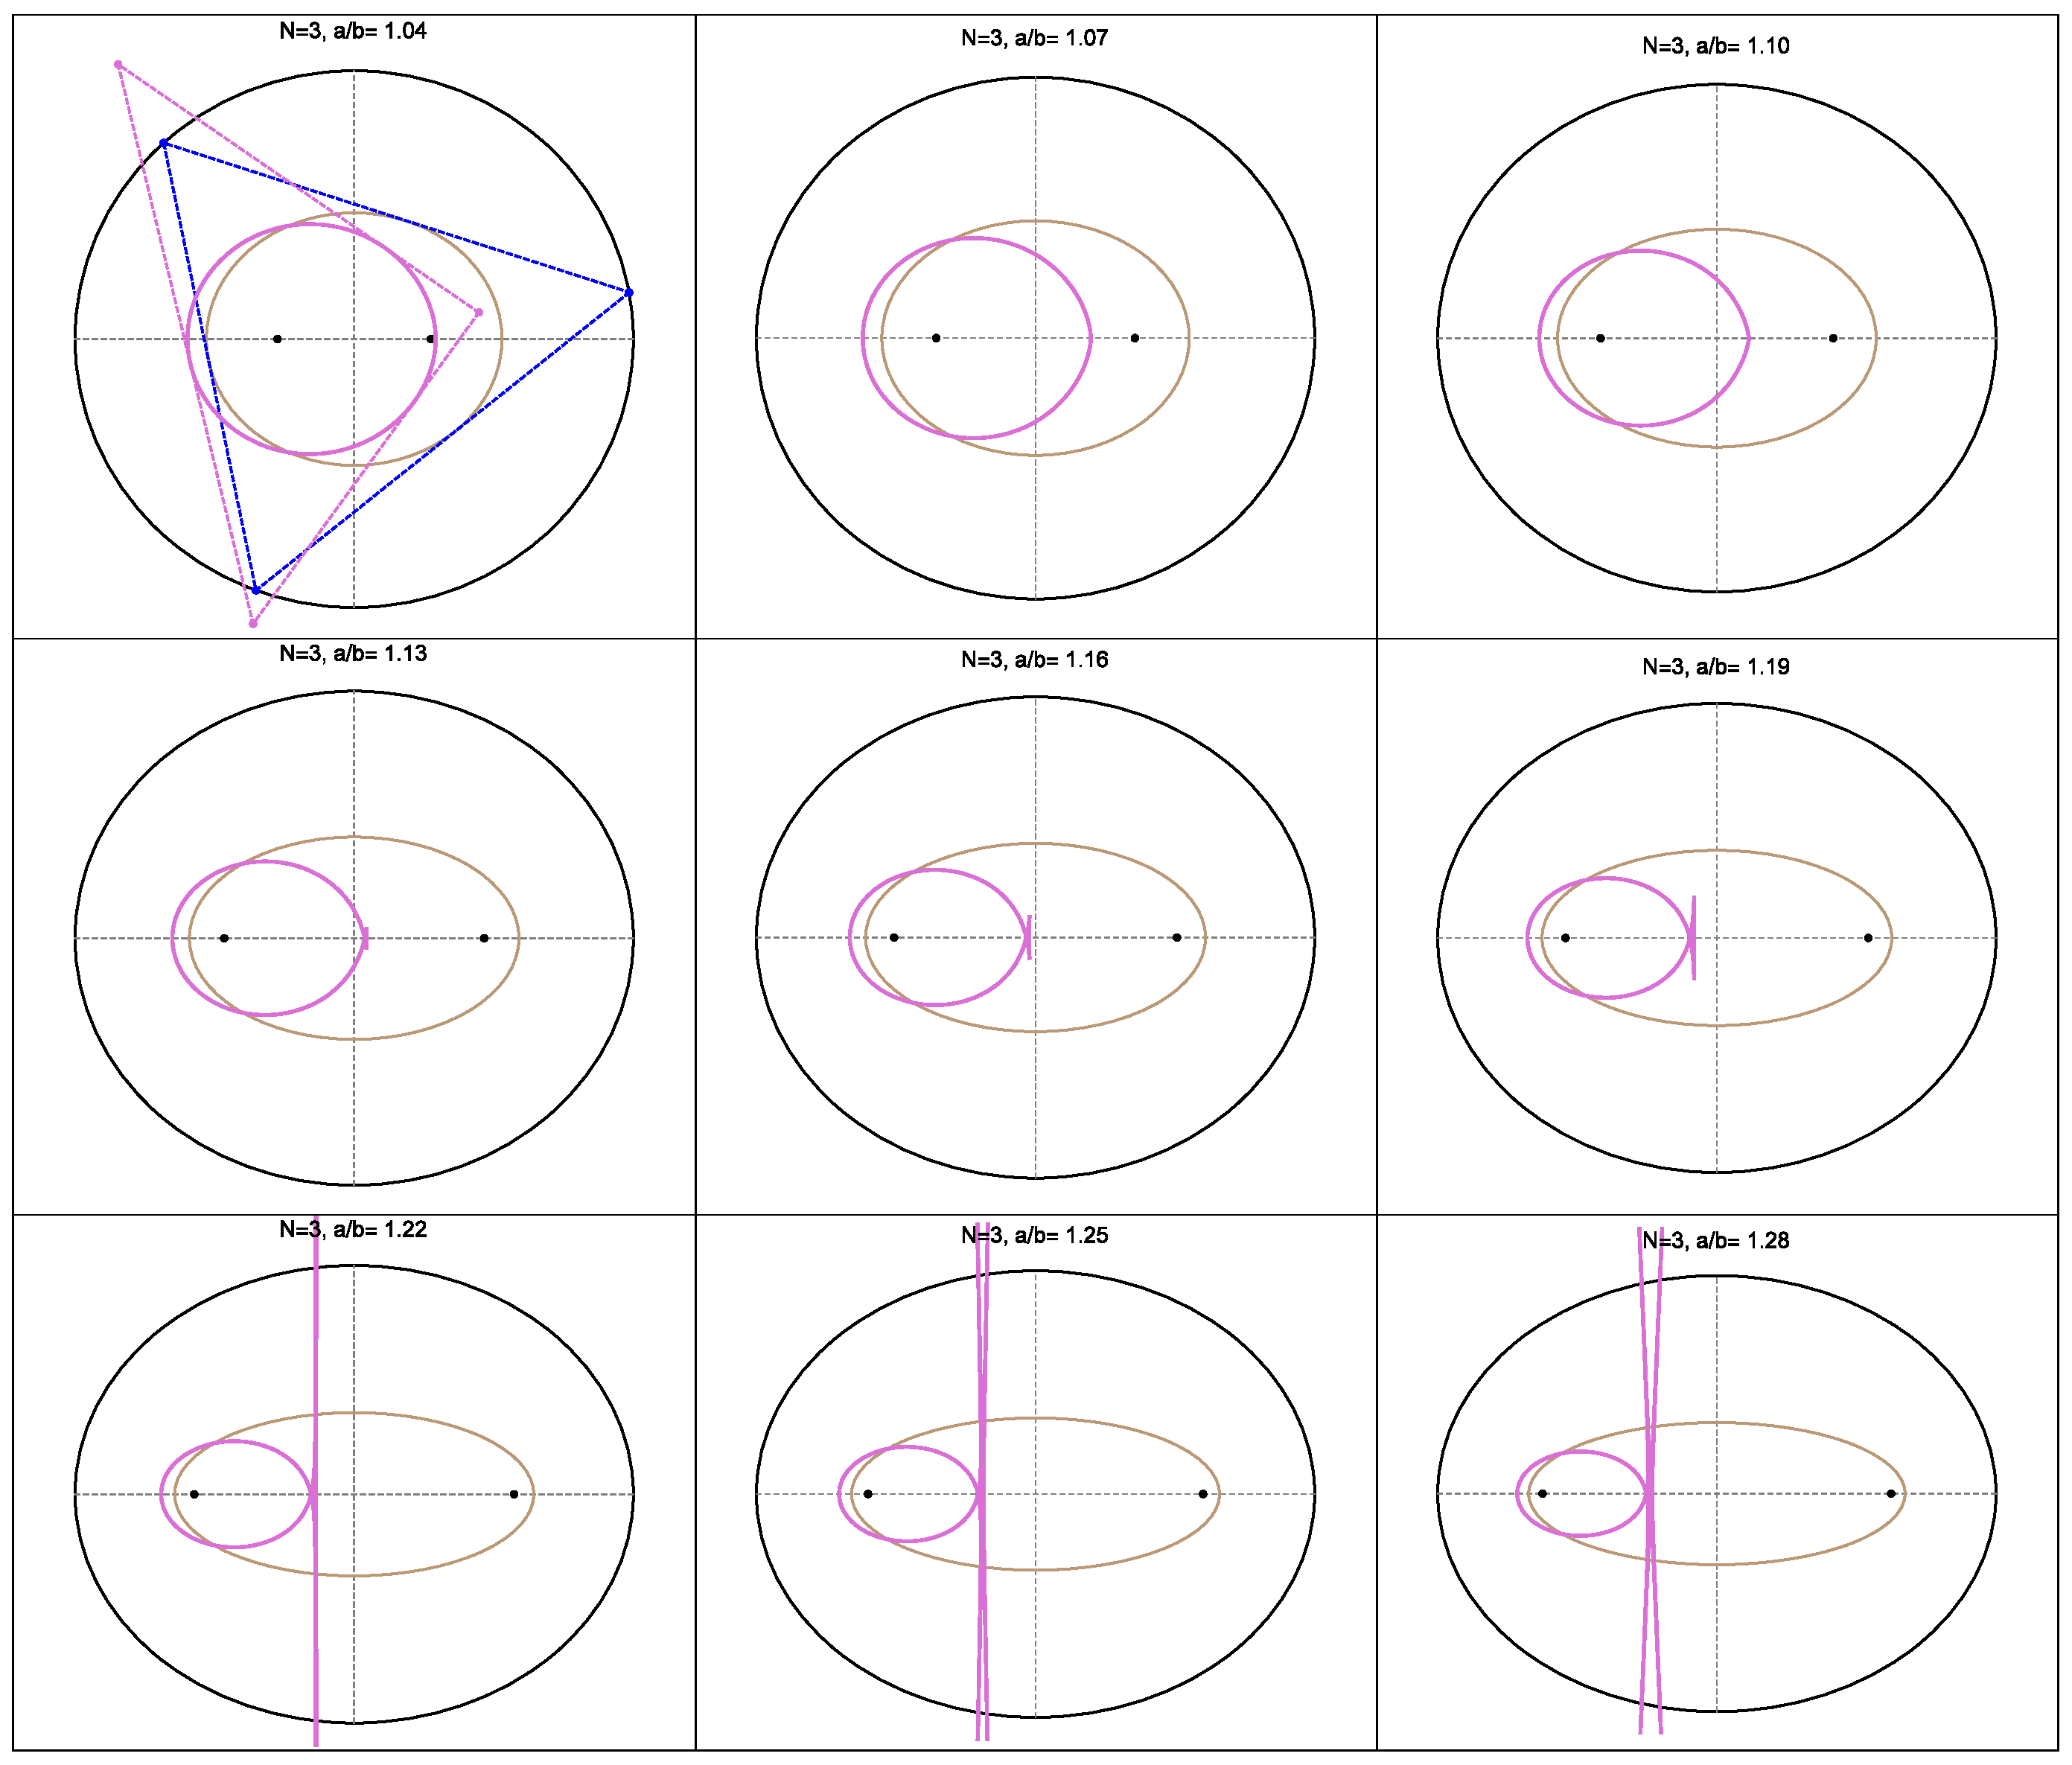
\includegraphics[width=\textwidth]{pics_08_020_n3_caustic.eps}
    \caption{Non-conic caustic (pink) to the focus-inversive family (pink). A billiard 3-periodic (dashed blue) and the corresponding focus-inversive triangle are shown at the top-left picture only. The billiard caustic is shown on every frame (brown). From left-to-right, top-to-bottom, $a/b$ is increased in small steps. Over this range, the caustic transitions from (i) a regular curve, to (ii) a curve with one self-intersection and two cusps, to (iii) a non-compact curve.  \href{https://bit.ly/374jbBl}{Live}}
    \label{fig:08-n3-caustics}
\end{figure}

\section{A stationary point}

Recall in the confocal family the Mittenpunkt $X_9$ is stationary. Henceforth we shall append a $\dagger$ to all quantities referring to the focus-inversive family. Let $a,b$ denote the semi-axes of the pre-inversion billiard which we assume to be centered on $[0,0]$ and be axis-parallel to $x$, and $y$ respectively. Let $\rho$ denote the radius of $f_1=[-c,0]$, the (left) focus-centered inversion circle, $c^2=a^2-b^2$. Interestingly:

\begin{proposition}
The Gergonne point $X_7^\dagger$ of focus-inversives is stationary on the major axis of the pre-image confocal pair. Its coordinates are given by:
\[ X_7^\dagger=\left[c\left(1-\frac{\rho^2}{\delta+c^2}\right),0\right]\]
where as before: $\delta^2=a^4-(a b)^2+b^4$.
\label{prop:08-gergonne}
\end{proposition} 

\section{Billiard-like invariants}

The following two surprising invariants -- constant perimeter and sum of cosines -- are analogues to those displayed by billiard 3-periodics. Interestingly they are not consequences of elementary principles or transformations. 

\begin{proposition}
The perimeter $L^\dagger$ of focus-inversives is invariant and given by: 
\[L^\dagger=\rho^2 \frac {\sqrt { \left( 8\,{a}^{4}+4\,{a}^{2}{b}^{2}+2\,{b}^{4}
 \right) \delta+8\,{a}^{6}+3\,{a}^{2}{b}^{4}+2\,{b}^{6}}}{{a}^{2}{b}^{
2}}\]
\label{prop:08-inv-perimeter}
\end{proposition}

Let $\theta_i^\dagger$ denote angles internal to focus-inversives. 

\begin{proposition}
The sum of internal angle cosines of focus-inversives is invariant and given by: 
\[
\sum\cos{\theta_{1,i}^\dagger}=\frac{\delta (a^2+c^2-\delta)}{a^2c^2} \]
\label{prop:08-inv-cos-sum}
\end{proposition}

\section{The rotating billiard table}

Recall that in \cref{fig:02-circumbilliard} we introduced the concept of the {\em circumbilliard}: given a triangle $T$, this is the $X_9$-centered circumellipse of which $T$ is a billiard 3-periodic (circumellipse normals are angular bisectors). Let  $\mathcal{C}^\dagger$ denote the (moving) circumbilliard ($X_9^\dagger$-centered circumellipse) of focus-inversives. Indeed, and referring to \cref{fig:08-moving-billiard-table}, focus-inversives are billiard 3-periodics of a rigidly-moving virtual elliptic billiard (see \cref{exe:08-moving-billiard-table}):

\begin{proposition}
Over focus-inversives, the semi-axes $a^\dagger,b^\dagger$ of $\mathcal{C}^\dagger$ are invariant and given by:

\begin{align*}
    a^\dagger&= \rho\,k_1
\sqrt {k_2\left(\delta+a\,c\right)}\\
    b^\dagger&= \rho\,k_1
\sqrt {k_2\left(\delta-a\,c\right) }\\
 \mbox{where:}&\\
k_1&=\frac{c \sqrt{2}}{k_3}\sqrt { \left( 8\,{a}^{4}+4\,{a}^{2}{b}^{2}+2\,{b}^{4}
 \right) \delta+8\,{a}^{6}+3\,{a}^{2}{b}^{4}+2\,{b}^{6}}\\
 k_2&=2 a^2-b^2-\delta\\
 %\sqrt{ \left( -4\,{a}^{2}+2\,{b}^{2} \right) \delta+5\,{a}^{4}-5\,{a}^{2}{b}^{2}+2\,{b}^{4}}\\
k_3&=2a  {b}^{2} \left(  \left( 2\,{a}^{2}-{b}^{2} \right) \delta+2
\,{a}^{4}-2\,{a}^{2}{b}^{2}-{b}^{4}\right)
\end{align*}
\end{proposition}

\begin{figure}
    \centering
    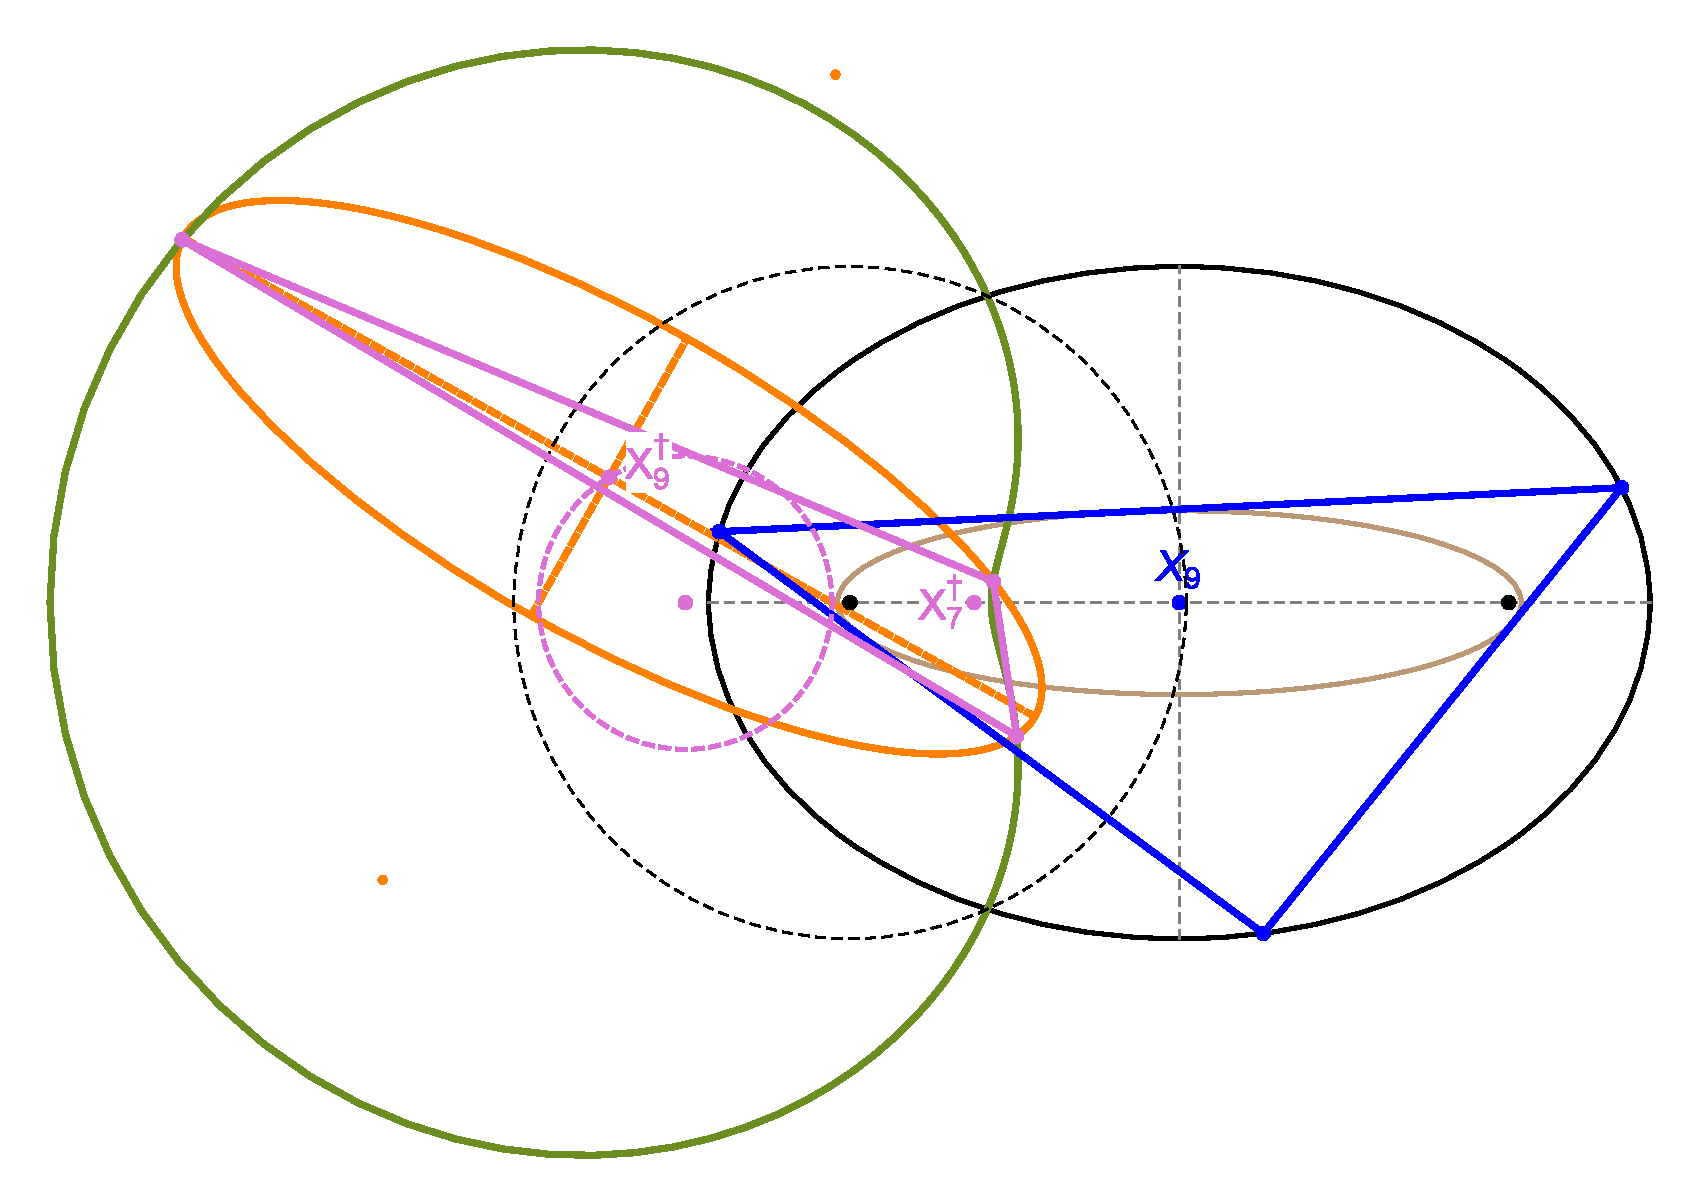
\includegraphics[width=\textwidth]{pics_08_030_n3_rotating_billiard.eps}
    \caption{The moving circumbilliard (orange) to focus-inversives (pink) rigidly translate and rotate (invariant semi-axes). Their center $X_9^\dagger$ sweeps a circle. The location of the stationary Gergonne point $X_7^\dagger$ is also shown. \href{https://youtu.be/LOJK5izTctI}{Video 1}, \href{https://youtu.be/Y-j5eXqKGQE}{Video 2}}
    \label{fig:08-n3-moving-billiard-table}
\end{figure}

\section{Invariant area product}

Let $A_1^\dagger$ (resp. $A_2^\dagger$) denote the area of the $f_1$- (resp. $f_2$) inversive triangle family. Referring to Figure~\ref{fig:08-inv-pedals}:

\begin{proposition}
For $N=3$, the area product $A_1^\dagger A_2^\dagger$ of the two focus-inversive triangles is given by:

\[ A_1^\dagger A_2^\dagger= \frac{\rho^8}{8 a^8 b^2}  \left[\left( {a}^{4}+2\,{a}^{2}{b}^{2}+4\,{b}^{4} \right)\delta +  \frac{3 a^{4} b^{2}}{2}+a^6+4\,{b}^{6} \right]
\]
\end{proposition}

\begin{figure}
    \centering
    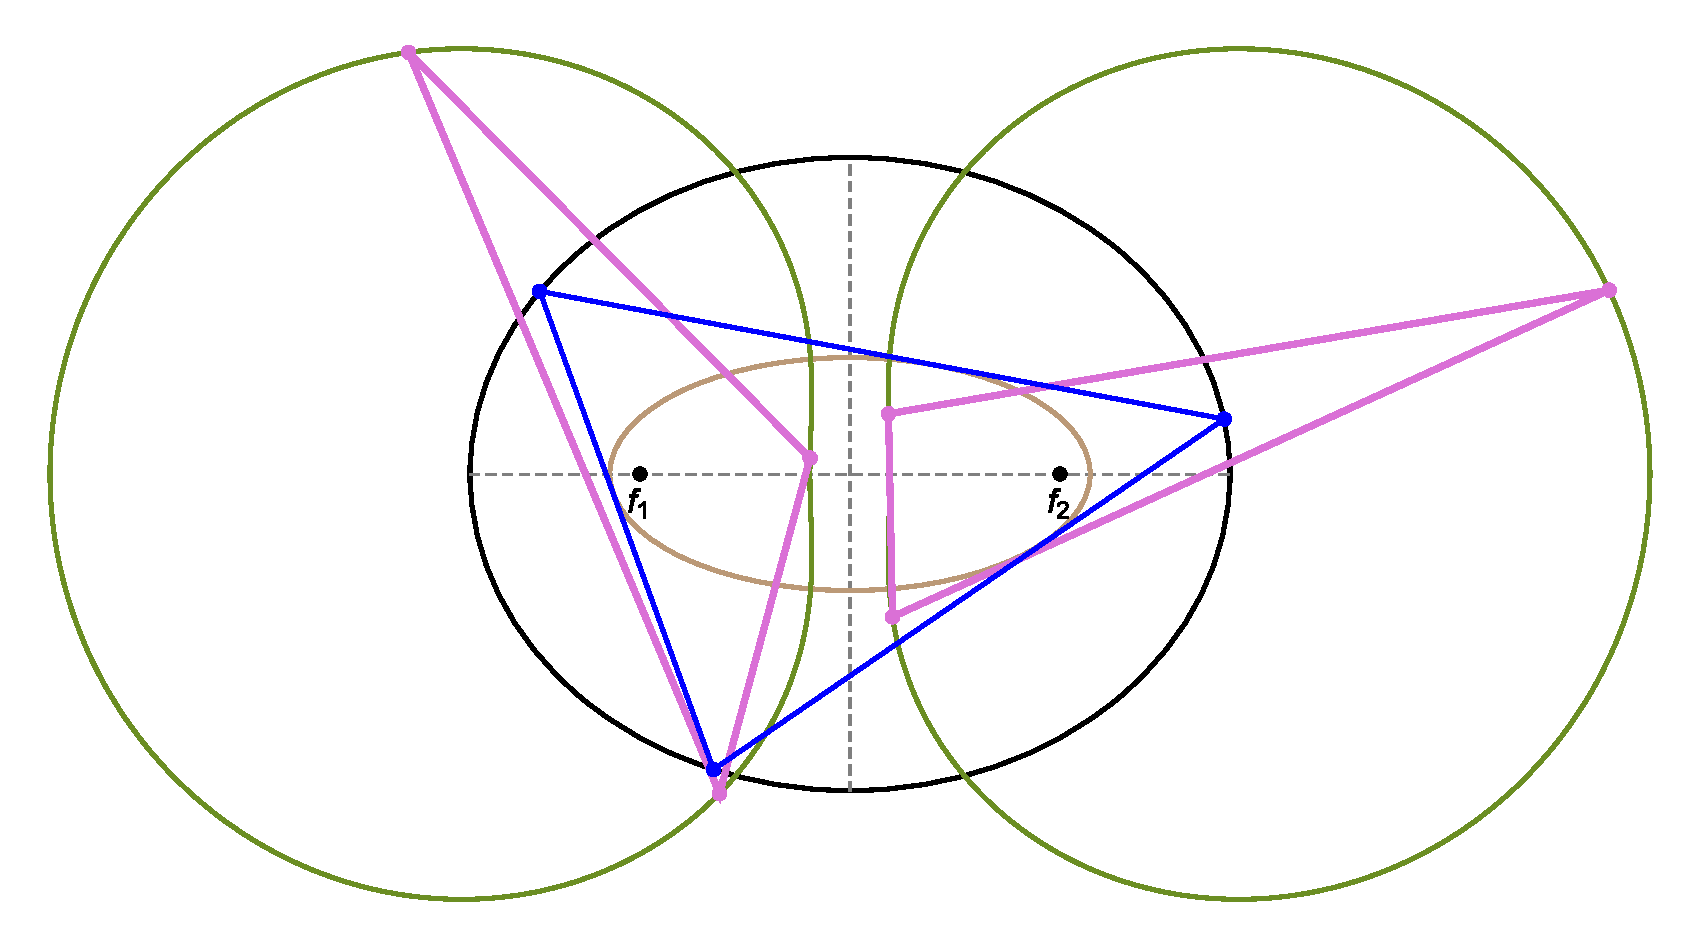
\includegraphics[width=\textwidth]{pics_08_040_n3_f1f2.eps}
    \caption{The area product of $f_1$- and $f_2$-inversive triangles (pink) is invariant. \href{https://youtu.be/0L2uMk2xyKk}{Video}, \href{https://bit.ly/3i1iPCM}{Live}}
    \label{fig:08-inv-pedals}
\end{figure}

\section{Circular loci galore!}

\begin{figure}
    \centering
    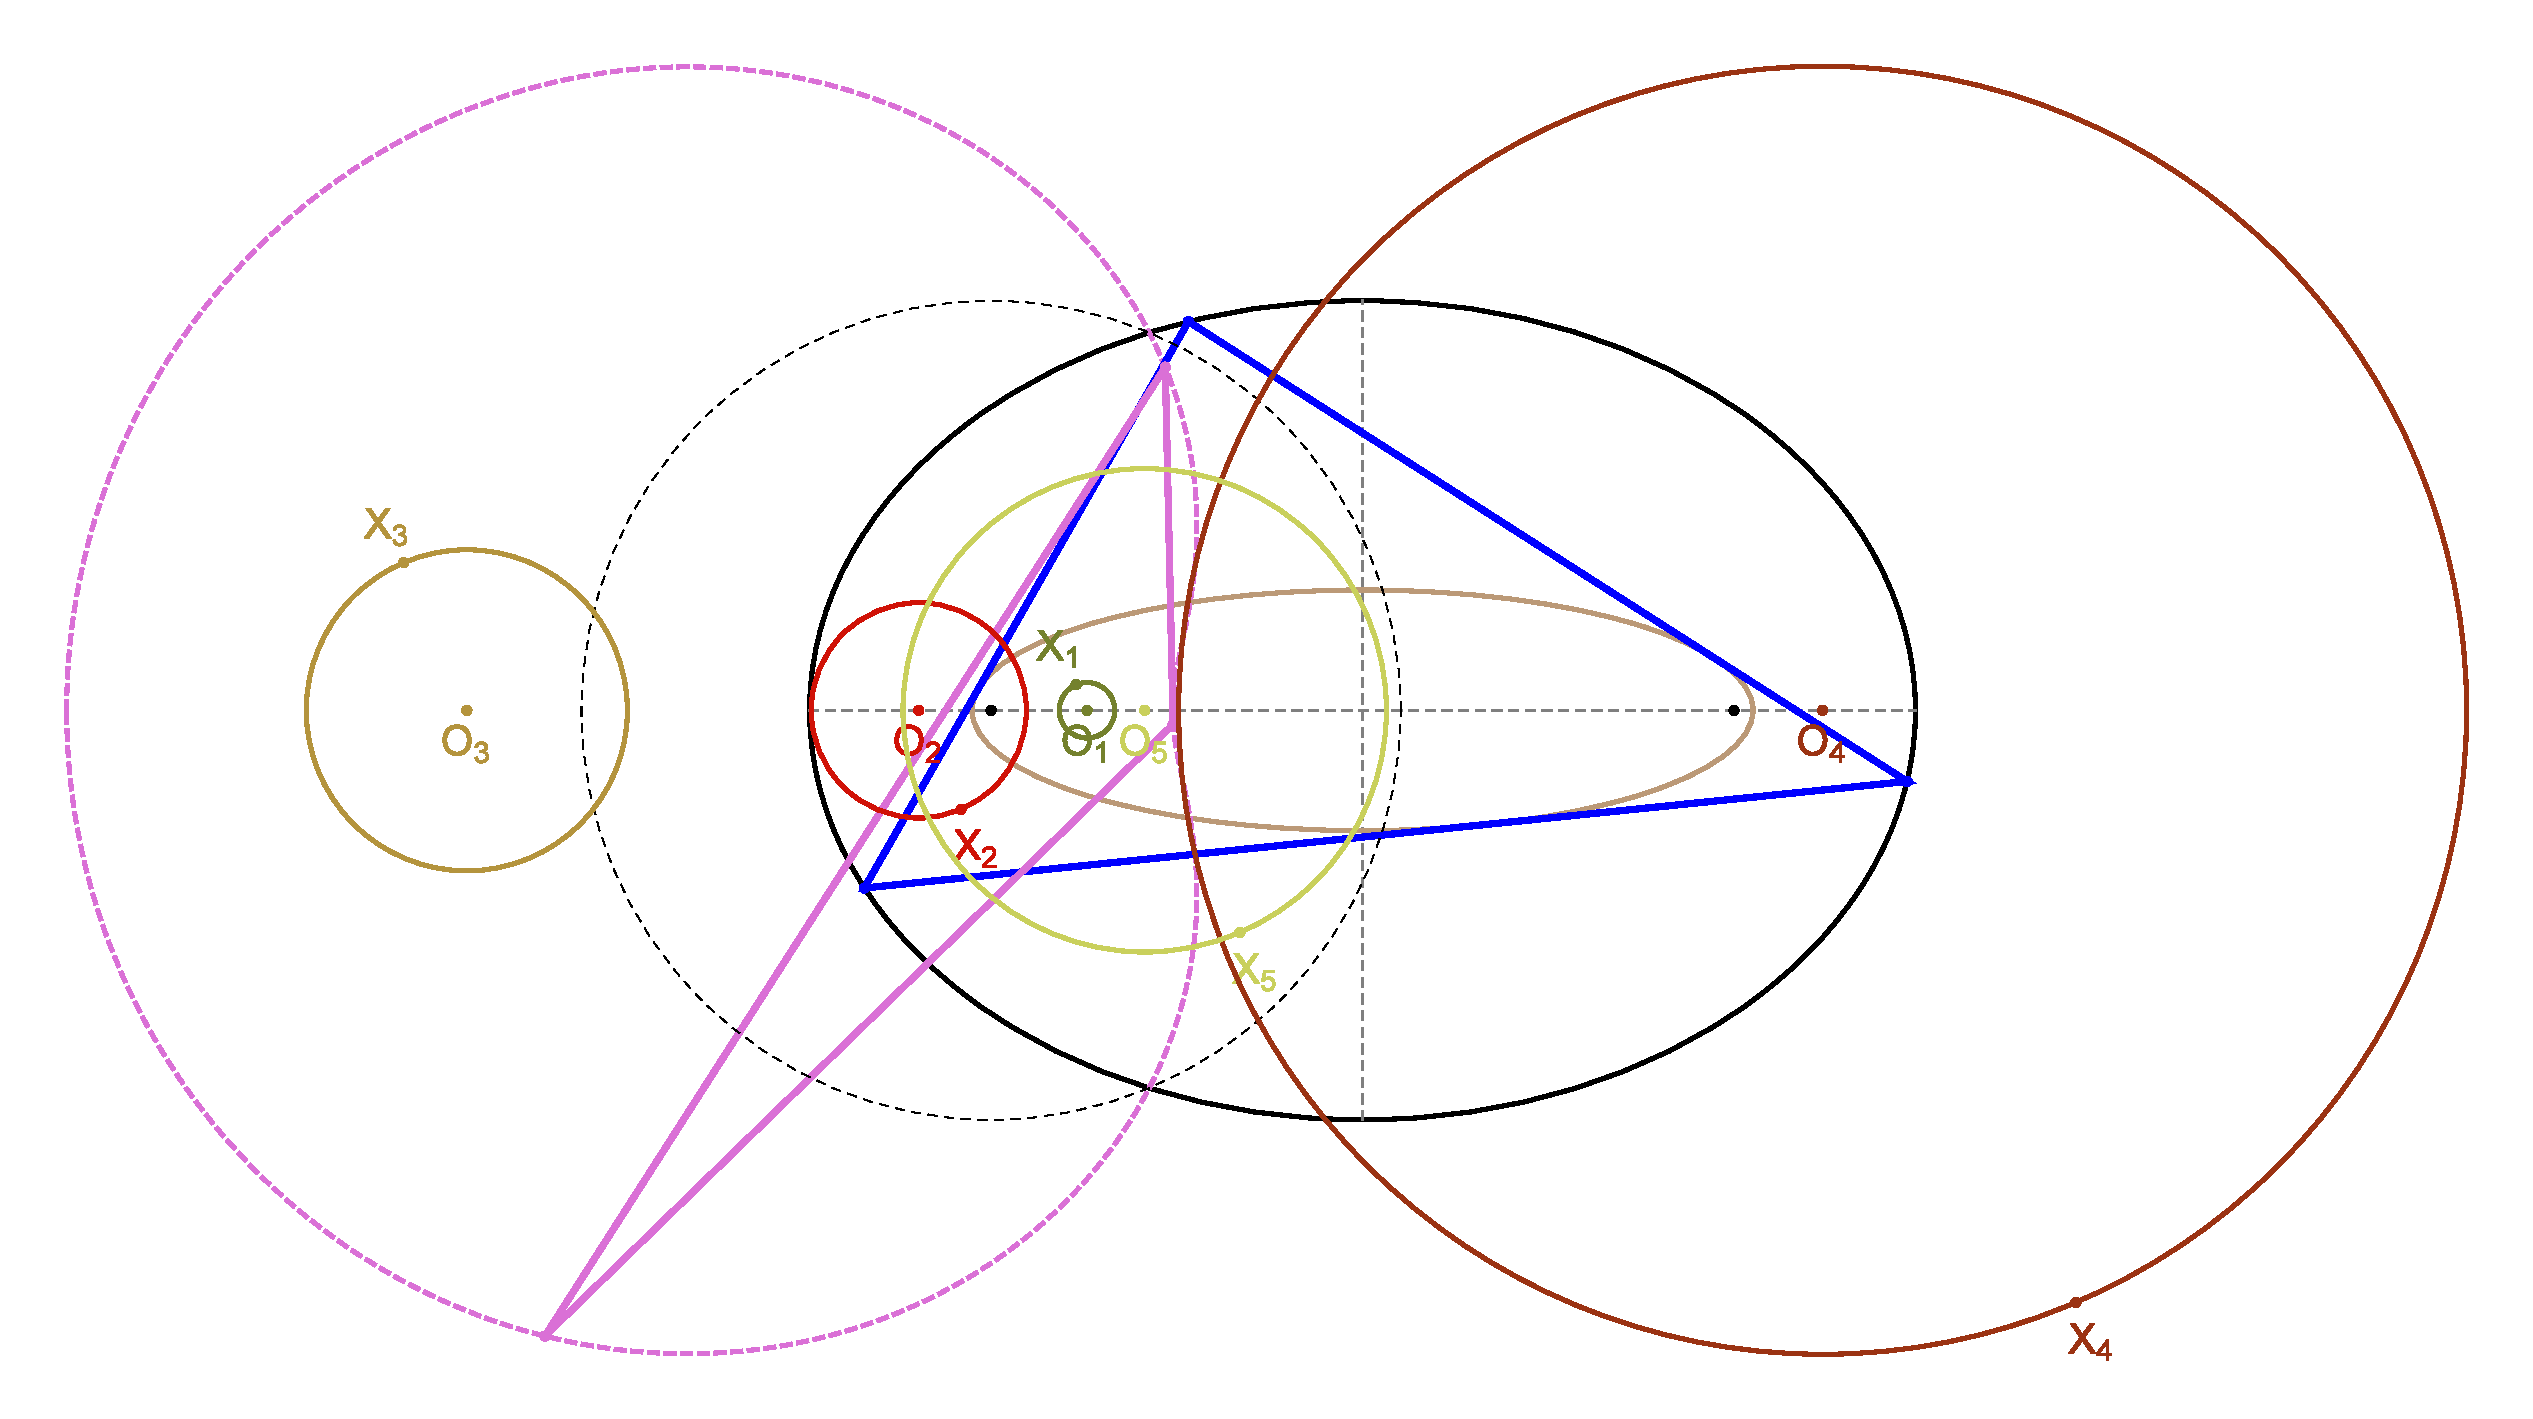
\includegraphics[width=\textwidth]{pics_08_050_n3_inv_loci12345}
    \caption{A focus-inversive 3-periodic (pink) is shown inscribed in Pascal's Limaçon (dashed pink). Also shown are the circular loci of $X_k^\dagger$, $k=1,2,3,4,5$ whose centers $O_i$ all lie on the billiard's major axis. \href{https://youtu.be/OAD2hpCRgCI}{Video}, \href{https://bit.ly/3fW3W1A}{Live}}
    \label{fig:08-n3-loci-12345}
\end{figure}

One remarkable property of focus-inversives is its ability to produce circular loci. Referring to Figure~\ref{fig:08-n3-loci-12345}:

\begin{proposition}
The locus of $X_1^\dagger$ is the circle given by:
\begin{align*}
C_1^\dagger=&\left[c\left(-1+\rho^2\frac{-2a^2+b^2+2\delta}{2b^4}\right), 0\right]\\
R_1^\dagger=&\rho^2\frac{-2\delta^2+b^4+(2a^2-b^2)\delta}{2ab^4}
\end{align*}
\end{proposition}

\begin{proposition}
The locus of $X_2^\dagger$ is the circle given by:

\begin{align*}
C_2^\dagger&=\left[-c\left(1+\rho^2\frac{2a^2-b^2-\delta}{3 a^2 b^2}\right),0\right]\\
R_2^\dagger&=\rho^2\frac{2 a^2-b^2-\delta}{3 a b^2}
\end{align*}
\end{proposition}

\begin{proposition}
The locus of $X_3^\dagger$ is the circle given by:
\begin{align*}
C_3^\dagger=&\left[-c\left(1+\rho^2\frac{a^2+b^2}{2b^4}\right), 0\right]\\
R_3^\dagger=&\rho^2\frac{a(-b^2+\delta)}{2b^4}
\end{align*}
\end{proposition}

\begin{proposition}
The locus of $X_4^\dagger$ is the circle given by:
\begin{align*}
C_4^\dagger=&\left[c\left(-1+\rho^2\frac{(b^2+\delta) \delta}{a^2 b^4}\right), 0\right]\\
R_4^\dagger=&\rho^2\frac{c^2(b^2+\delta)}{a b^4}
\end{align*}
\end{proposition}

\begin{proposition}
The locus of $X_5^\dagger$ is the circle given by:
\begin{align*}
C_5^\dagger=&\left[c\left(-1+ \rho^2\frac{a^4 - 3 a^2 b^2+2 b^4 + 2 b^2 \delta}{4 a^2 b^4}\right), 0\right]\\
R_5^\dagger=&\rho^2\frac{(3a^2-2b^2)b^2+(a^2-2b^2)\delta}{4a b^2}
\end{align*}
\end{proposition}

In \cref{sec:06-loci-types}, 42 triangle centers are identified (from within the first 200 on \cite{etc}), whose loci over billiard 3-periodics are ellipses. Interestingly:

\textcolor{red}{stopped here, need to determine if $X_{190}$ is non-monotonic}

\begin{observation}
Amongst the first 200 triangle centers listed on \cite{etc}, the following triangle centers $X_k^\dagger$ sweep conics over the focus-inversive family:

\begin{itemize}
\item Circles (40): 1,2,3,4,5,8,9,10,11,12,20,21,35,36,40,46,55,56,57,63,65,72,78, 79,80,84,90,100,104,119,140,142,144,145,149,150,153,165,191,200.
\item Ellipses (4): 69,75,85,86.
\item Hyperbolas (3): 47,49,91.
\end{itemize}
\end{observation}

Comparing these with conic locus centers in \cref{sec:06-loci-types}, one realizes that the only ones missing are $X_k$, $k=$88, 162, 190, called ``swans'' in \cref{sec:05-swans}: triangle centers which by construction lie on the $X_9$-centered circumellipse. In particular,  $X_{88}$ and $X_{162}$ were identified as non-monotonic swans, see \cref{sec:05-non-monotonic}. The monotonic swan $X_{100}$ does appear on the list below. Also missing is $X_{190}$, a swan whose monot

Through painstaking CAS-assisted simplification, we were able to obtain compact expressions for only a few of the above circular loci, namely: $X_k,k=$1, 2, 3, 4, 5, 9, 11, 100. 

Referring to Figure~\ref{fig:x159-x934}:

\begin{observation}
Amongst all 29 triangle centers whose loci are ellipses over billiard 3-periodics, only $X_{88}^\dagger$ does not sweep a circular locus over the focus-inversive family. Nevertheless, this locus is algebraic, regular, can be both convex and concave, and is symmetric wrt the major axis of the ellipse.
\end{observation}
